\subsection{PARACOMPACTNESS OF METRIZABLE SPACES}

The following theorem sharpens the result of Proposition 2 of no. 1:

THEOREM 4. Every metrizable space is paracompact.

The theorem is a consequence of the following four lemmas.

LEMMA 3. Let \(\Re = (U_{\alpha})_{\alpha \in A}\) be an open covering of a metrizable space \(X\) . Then there is a sequence \((\mathfrak{S}_n)\) of locally finite families of open subsets of \(X\) , such that \(\mathfrak{S} = \bigcup \mathfrak{S}_n\) is an open covering of \(X\) which refines \(\Re\) .

Let \(d\) be a metric on \(\mathbf{X}\) compatible with its topology. For each \(\alpha \in \mathbf{A}\) and each integer \(n\) , let \(\mathbf{F}_{n\alpha}\) denote the set of all \(x \in \mathbf{U}_{\alpha}\) such that \(d(x, \mathbf{X} - \mathbf{U}_{\alpha}) \geqslant 2^{-n}\) . Since \(\mathbf{X} - \mathbf{U}_{\alpha}\) is closed, we have \(\mathbf{U}_{\alpha} = \bigcup_{n} \mathbf{F}_{n\alpha}\) . Well-order the set \(\mathbf{A}\) ; for each \(\alpha \in \mathbf{A}\) and each integer \(n\) , let \(\mathbf{G}_{n\alpha}\) be the set of all \(x \in \mathbf{F}_{n\alpha}\) such that \(x \notin \mathbf{F}_{n+1,\beta}\) for all \(\beta < \alpha\) , and let \(\mathbf{V}_{n\alpha}\) be the set of all \(y \in \mathbf{X}\) such that \(d(y, \mathbf{G}_{n\alpha}) - 2^{-n-3}\) . \(\mathbf{V}_{n\alpha}\) is clearly an open set; on the other hand, \(\mathbf{V}_{n\alpha} \subset \mathbf{U}_{\alpha}\) , because for each \(y \in \mathbf{V}_{n\alpha}\) there exists \(x \in \mathbf{G}_{n\alpha}\) such that \(d(x, y) \leqslant 2^{-n-1}\) , and since \(x \in \mathbf{F}_{n\alpha}\) , we have

\[
d (y, \mathrm{X} - \mathrm{U} _ {\alpha}) \geqslant d (x, \mathrm{X} - \mathrm{U} _ {\alpha}) - d (x, y) \geqslant 2 ^ {- n - 1},
\]

so that \(y \in \mathbf{U}_{\alpha}\) . Furthermore, for each \(x \in \mathbf{X}\) let \(\alpha\) be the smallest index in \(\mathbf{A}\) such that \(x \in \mathbf{U}_{\alpha}\) ; then there is an integer \(n\) such that \(x \in \mathrm{F}_{n\alpha}\) , and the definition of \(\alpha\) implies that \(x \in \mathrm{G}_{n\alpha}\) , so that \(x \in \mathrm{V}_{n\alpha}\) . This shows that if we put \(\mathfrak{S}_n = (\mathrm{V}_{n\alpha})_{\alpha \in \mathbf{A}}\) , then \(\mathfrak{S} = \bigcup_{n} \mathfrak{S}_n\) is an open

covering of X which refines \(\Re\) ; thus it remains to be shown that each of the families \(\mathfrak{S}_n\) is locally finite. To this end we shall first show that \(d(\mathrm{G}_{n\alpha}, \mathrm{G}_{n\beta}) \geqslant 2^{-n-1}\) if \(\alpha \neq \beta\) . Suppose that \(\beta < \alpha\) ; then if \(x \in \mathrm{G}_{n\alpha}\) and \(y \in \mathrm{F}_{n\beta}\) we have \(x \notin \mathrm{F}_{n+1, \beta}\) by definition, hence \(d(x, \mathrm{X} - \mathrm{U}_{\beta}) < 2^{-n-1}\) and \(d(y, \mathrm{X} - \mathrm{U}_{\beta}) \geqslant 2^{-n}\) , and therefore \(d(x, y) \geqslant 2^{-n-1}\) ; since \(\mathrm{G}_{n\beta} \subset \mathrm{F}_{n\beta}\) , the assertion follows. From this it follows immediately, using the definition of \(\mathrm{V}_{n\alpha}\) and \(\mathrm{V}_{n\beta}\) , that \(d(\mathrm{V}_{n\alpha}, \mathrm{V}_{n\beta}) \geqslant 2^{-n-2}\) . From this last inequality we deduce that, for each \(z \in \mathrm{X}\) , the open ball with centre \(z\) and radius \(2^{-n-3}\) meets at most one set of the family \(\mathfrak{S}_n\) ; hence \(\mathfrak{S}_n\) is a locally finite family, and the proof is complete.

LEMMA 4. Let \((\mathfrak{S}_n)\) be a sequence of locally finite families of open sets in a topological space \(\mathbf{X}\) , such that

\[
\mathfrak {S} = \bigcup_ {n} \mathfrak {S} _ {n}
\]

is a covering of X. Then there exists a locally finite (but not necessarily open) covering B of X which refines S.

Let \(\mathbf{E}_n\) be the open set in \(\mathbf{X}\) which is the union of all the sets of \(\mathfrak{S}_n\) ;

let \(U_{n}\) denote \(\bigcup_{k=1}^{n}E_{k}\) and let \(A_{n}\) denote \(U_{n}-U_{n-1}\) (with \(U_{0}=\varnothing\) ). Consider the set B of subsets \(V\cap A_{n}\) , where \(V\in S_{n}\) and n is any integer; we shall show that B satisfies the conditions of the lemma. For each \(x\in X\) there is an integer n such that \(x\in A_{n}\) , since the \(A_{n}\) form a partition of X; thus \(x\in E_{n}\) and there exists \(V\in S_{n}\) such that \(x\in V\) ; so \(x\in V\cap A_{n}\) , and we have proved that B is a covering of X. Clearly, this covering refines S. On the other hand, for each \(x\in X\) there exists an integer n such that \(x\in U_{n}\) ; since \(U_{n}\) is open and the \(S_{m}\) are locally finite families, there exists a neighbourhood \(W_{m}\) of x, for each m, contained in \(U_{n}\) , which meets only a finite number of sets of \(S_{m}\) ; hence the neighbourhood \(W=\bigcap_{m=1}^{n}W_{m}\) of x meets only a finite number of sets of B, because \(W\cap A_{p}=\varnothing\) for p\textgreater n.~Hence B is locally finite, and Lemma 4 is proved.

LEMMA 5. Let X be a regular space such that, for each open covering R of X, there exists a (not necessarily open) locally finite covering A of X which refines R. Then for each open covering R of X there exists a locally finite closed covering F of X which refines R.

Let \(\mathfrak{R}\) be any open covering of X. For each \(x \in \mathbf{X}\) there is an open set \(\mathbf{U} \in \mathfrak{R}\) which contains \(x\) , and therefore (since X is regular) an open neighbourhood \(\mathbf{V}_x\) of \(x\) such that \(\overline{\mathbf{V}}_x \subset \mathbf{U}\) . The family \(\mathfrak{B}\) formed by the \(\mathbf{V}_x\) is an open covering of X, hence by hypothesis there is a locally finite covering \(\mathfrak{B}\) which is finer than \(\mathfrak{B}\) . Let \(\mathfrak{F}\) be the family of closures of the sets of \(\mathfrak{B}\) . Since the covering \(\mathfrak{B}'\) formed by the \(\overline{\mathbf{V}}_x\) is finer than \(\mathfrak{R}\) , and since \(\mathfrak{F}\) is finer than \(\mathfrak{B}'\) , it follows that \(\mathfrak{F}\) is a closed covering of X which refines \(\mathfrak{R}\) . But also \(\mathfrak{F}\) is locally finite, because if an open set does not meet a set \(\mathbf{B} \in \mathfrak{B}\) , then it does not meet its closure \(\overline{\mathbf{B}}\) either.

LEMMA 6. Let X be a Hausdorff space such that, given any open covering R of X, there exists a locally finite closed covering F of X which refines R. Then X is paracompact.

Let \(\mathfrak{R}\) be any open covering of X. We have to show that there is a locally finite open covering of X which refines \(\mathfrak{R}\) . Let \(\mathfrak{A}\) be a locally finite covering (closed or not) of X which refines \(\mathfrak{R}\) ; for each \(x \in \mathbf{X}\) , let \(W_x\) be an open neighbourhood of \(x\) which meets only a finite number of sets of \(\mathfrak{A}\) . The family \(\mathfrak{B}\) of sets \(W_x\) is an open covering of X. Let \(\mathfrak{F}\) be a locally finite closed covering of X which refines \(\mathfrak{B}\) . For each \(A \in \mathfrak{A}\) , let \(U_A\) be a set of \(\mathfrak{R}\) which contains A, and let \(C_A\) be the union of the sets \(F \in \mathfrak{F}\) such that \(A \cap F = \emptyset\) . Since \(\mathfrak{F}\) is locally finite, \(C_A\) is closed in X (Chapter I, § 1, no. 6, Proposition 4) and therefore \(A' = U_A \cap (X - C_A)\) is open. Since we have \(A \cap C_A = \emptyset\) and \(A \subset U_A\) , it follows that \(A \subset A'\) , and the family \(\mathfrak{A}'\) of sets \(A'\) , as A runs through \(\mathfrak{A}\) , is an open covering of X; moreover, since \(A' \subset U_A \in \mathfrak{R}\) , \(\mathfrak{A}'\) refines \(\mathfrak{R}\) . It remains to show that \(\mathfrak{A}'\) is locally finite. For each \(x \in X\) there is a neighbourhood T of \(x\) which meets only a finite number of sets of \(\mathfrak{F}\) , say \(F_1, \ldots, F_n\) . Since each \(F_i\) is contained in a set of the form \(W_{y_i}\) , by definition \(F_i\) meets only a finite number of sets of \(\mathfrak{A}\) ; let \(A_{ij} (i \leqslant j \leqslant s_i)\) be these sets. If A is a set of \(\mathfrak{A}\) other than one of the \(A_{ij} (i \leqslant i \leqslant n, i \leqslant j \leqslant s_i)\) , it follows from the definitions that \(A'\) meets none of the \(F_i\) , and therefore does not meet \(T \subset \bigcup_{i=1}^{n} F_i\) . This completes the proof of Lemma 6 and of Theorem 4.

\section{BAIRE SPACES}

\subsection{NOWHERE DENSE SETS}

DEFINITION 1. A subset A of a topological space X is said to be nowhere dense if its closure has no interior points.

Equivalently, A is nowhere dense in X if and only if the exterior of A is dense in X.

A closed set A is nowhere dense if and only if it has no interior points; that is, if and only if it coincides with its frontier. An arbitrary subset A is nowhere dense if and only if the closure of A is nowhere dense. Every subset of a nowhere dense set is nowhere dense.

Examples. 1) The empty subset of X is nowhere dense. In a Hausdorff space X, a set consisting of a single point is nowhere dense if and only if the point is not isolated in X. A dense subset is never nowhere dense (unless \(X = \varnothing\) ).

\begin{enumerate}
\def\labelenumi{\arabic{enumi})}
\setcounter{enumi}{1}
\item
  The frontier of an open or of a closed set is always nowhere dense.
\item
  In the space \(\mathbf{R}^n\) , every linear subspace of dimension \(p < n\) is a nowhere dense set (Chapter VI, § 1, no. 4, Proposition 2).
\end{enumerate}

Remark. The frontier of an arbitrary subset need not be nowhere dense: for example, if A and \(\mathbb{C}\) A are both dense sets, then the frontier of A is the whole space.

PROPOSITION I. The union of a finite number of nowhere dense sets is nowhere dense.

It is enough to show that the union of two nowhere dense sets A, B is nowhere dense, and without loss of generality we may assume that A and B are closed. The proposition is then equivalent to saying that the intersection of two dense open sets CA, CB is dense. Now if U is a non-empty open set, then \(U \cap CA\) is open and non-empty, hence

\[
\left(\mathrm{U} \cap \mathbb {C A}\right) \cap \mathbb {C B} = \mathrm{U} \cap \left(\mathbb {C A} \cap \mathbb {C B}\right)
\]

is open and non-empty.

Let Y be a subspace of a topological space X. A subspace A of Y is said to be nowhere dense relative to Y if A is nowhere dense when considered as a subset of the topological space Y.

PROPOSITION 2. Let Y be a subspace of a topological space X, and let A be a subset of Y. If A is nowhere dense relative to Y, then A is nowhere dense relative to X. Conversely, if Y is open in X and A is nowhere dense relative to X, then A is nowhere dense relative to Y.

Suppose that A is nowhere dense relative to Y. If the closure \(\overline{A}\) of A in X contains a non-empty open set U, then \(U \cap A\) is not empty (by the definition of closure); hence \(U \cap Y\) is a non-empty open set relative to Y, and is contained in the closure \(\overline{A} \cap Y\) of A with respect to Y, which is contrary to the hypothesis.

Now suppose that Y is open in X and that \(A \subset Y\) is nowhere dense relative to X. If U is open in Y and is not empty, then U is open in X and therefore contains a non-empty set V which is open in X (and a fortiori in Y) and does not meet A; hence A is nowhere dense relative to Y.

The second part of Proposition 2 is clearly not valid if Y is not open in X; consider, e.g., the situation where \(Y \neq \varnothing\) is nowhere dense in X, and A = Y.

\subsection{MEAGRE SETS}

DEFINITION 2. A subset A of a topological space X is said to be meagre if it is the union of a countable family of nowhere dense sets.

Equivalently, A is meagre if it is contained in a countable union of closed sets each of which has no interior points.

A meagre set can perfectly well be dense in X; even the whole space X can itself be a meagre set.

An example of the latter possibility is provided by any countable Hausdorff space with no isolated points, e.g., the rational line Q. But a topological space X which is a meagreset in X need not be countable (see Exercise 9).

Every subset of a meagre set in a space X is meagre, and the union of a countable family of meagre sets is meagre.

Let Y be a subspace of X. A subset A of Y is said to be meagre relative to Y if A is meagre when considered as a subset of the topological space Y. It follows from Proposition 2 of no. 1 that if A is a subset of Y which is meagre relative to Y, then A is meagre relative to X; and that if also Y is open in X, every subset A of Y which is meagre relative to X is meagre relative to Y.

\subsection{BAIRE SPACES}

DEFINITION 3. A topological space X is said to be a Baire space if it satisfies one or the other of the following two equivalent conditions:

(EB) Every countable intersection of dense open sets in \(\mathbf{X}\) is dense in \(\mathbf{X}\) .

(EB') Every countable union of closed sets with no interior points in X has no interior point in X.

Axiom (EB) can be stated in two other equivalent forms:

(EB'') Every non-empty open set in X is non-meagre.

Indeed a set is meagre if and only if it is contained in a countable union of closed sets with no interior points.

(EB''\,``) The complement of a meagre set in X is dense in X.

This signifies that a meagre set cannot contain a non-empty open set, and is therefore equivalent to \((EB'')\) .

PROPOSITION 3. Every non-empty open subspace Y of a Baire space X is a Baire space.

This follows from (EB''), for every open (resp. meagre) set in Y is open (resp. meagre) in X.

It follows from Proposition 3 that every point of a Baire space has a fundamental system of neighbourhoods, each of which is a Baire space. Conversely:

PROPOSITION 4. If every point of a topological space X has a neighbourhood which is a Baire space, then X is a Baire space.

Let A be a non-empty open set in X, let \(x \subset A\) and let V be an open neighbourhood of x which is a Baire space. If A were meagre in X, then \(V \cap A\) would be meagre in V and open in V, which is contrary to hypothesis.

PROPOSITION 5. In a Baire space X, the complement of a meagre set is a Baire space.

Let A be a meagre set in X; then its complement Y = CA in X is dense in X. Let B be a meagre set relative to Y; B is also meagre relative to X, hence A ∪ B is meagre relative to X. Hence the complement of A ∪ B in X, which is also the complement of B in Y, is dense in X and a fortiori dense in Y. Hence Y is a Baire space.

THEOREM I (Baire). (i) Every locally compact space X is a Baire space. (ii) Every topological space X on which there exists a metric, compatible with the topology of X and which defines on X the structure of a complete metric space, is a Baire space.

We shall show that axiom (EB) is satisfied in each case. Let \((\mathbf{A}_n)\) be a sequence of dense open sets in \(\mathbf{X}\) , and let \(\mathbf{G}\) be any non-empty open set. We can then define inductively a sequence \((\mathbf{G}_n)\) of non-empty open sets such that \(\mathbf{G}_1 = \mathbf{G}\) and \(\overline{\mathbf{G}}_{n+1} \subset \mathbf{G}_n \cap \mathbf{A}_n\) : for since by hypothesis \(\mathbf{G}_n\) is not empty, \(\mathbf{G}_n \cap \mathbf{A}_n\) is a non-empty open set; and since \(\mathbf{X}\) is regular in both cases envisaged, there is a non-empty open set \(\mathbf{G}_{n+1}\) such that \(\overline{\mathbf{G}}_{n+1} \subset \mathbf{G}_n \cap \mathbf{A}_n\) . Hence the set \(\mathbf{G} \cap \bigcap_{n=1}^{\infty} \mathbf{A}_n\) contains the intersection of the sets \(G_{n}\) , which is equal to the intersection of the sets \(\overline{G}_{n}\) ; hence it is enough to show that \(\bigcap_{n=1}^{\infty}\overline{G}_{n}\neq\varnothing\) . Now if X is locally compact, we may assume that \(\overline{G}_{2}\) is compact; in the compact space \(\overline{G}_{2}\) , the \(\overline{G}_{n}(n\geqslant2)\) form a decreasing sequence of non-empty closed sets, and their intersection is therefore not empty by axiom (C'\,') (cf.~Chapter I, §9, no. 1, Definition 1{]}. If X is a complete metric space (with respect to a metric compatible with its topology) we may suppose that \(\overline{G}_{n}\) has been chosen so that its diameter (with respect to this metric) tends to o as n tends to \(+\infty\) ; the \(\overline{G}_{n}\) therefore form a Cauchy filter base which converges to a point x, and x necessarily belongs to the intersection of the sets \(\overline{G}_{n}\) . Q.E.D.

Remark. There are Baire spaces which belong to neither of these two categories, in particular Baire spaces which are neither metrizable nor locally compact (Exercise 16); there are also metrizable Baire spaces which possess no complete metric space structure compatible with their topology (Exercise 14).

\subsection{SEMI-CONTINUOUS FUNCTIONS ON A BAIRE SPACE}

THEOREM 2. Let X be a Baire space and let \((f_{\alpha})\) be a family of lower semi-continuous real-valued functions on X such that, at every point x of X, the upper envelope \(\sup_{\alpha} f_{\alpha}(x)\) is finite. Then every non-empty open set in X contains a non-empty open set on which the family \((f_{\alpha})\) is uniformly bounded above.

This theorem may also be stated in the form that the set of points in the neighbourhood of which the family \((f_{\alpha})\) is uniformly bounded above is a dense open set.

Let \(f = \sup_{\alpha} f_{\alpha}\) be the upper envelope of the family \((f_{\alpha})\) . The function \(f\) is lower semi-continuous (Chapter IV, § 6, no. 2, Theorem 4) and finite at every point of \(\mathbf{X}\) . It is therefore enough to carry through the proof in the case where the family \((f_{\alpha})\) consists of a single function \(f\) . Let \(\mathbf{A}_n\) be the set of points \(x \in \mathbf{X}\) such that \(f(x) \leqslant n\) ; \(\mathbf{A}_n\) is closed (Chapter IV, § 6, no. 2, Proposition 1), and the assumptions imply that \(\mathbf{X}\) is the union of the sets \(\mathbf{A}_n\) ; hence at least one of the \(\mathbf{A}_n\) has an interior point, and therefore there is a non-empty open set on which \(f\) is bounded above (by an integer \(n\) ). If we apply this result to any non-empty open subset of \(\mathbf{X}\) (this subspace is also a Baire space by Proposition 3 of no. 3), we have the theorem.

In applications of this theorem it is generally the case that the \(f_{\alpha}\) are continuous on X.

Remark. The theorem may be false if we do not suppose that X is a Baire space. For example if, for each rational number p/q (p, q being coprime integers, q \textgreater{} 0) we put \(f(p/q) = q\) , we have a lower semicontinuous function f on the rational line Q which is finite at each point (cf.~Chapter IV, § 6, no. 2); but there is no non-empty open set in Q on which f is bounded above.

\section{POLISH SPACES, SOUSLIN SPACES, BOREL SETS}

\subsection{POLISH SPACES}

DEFINITION 1. A topological space X is said to be Polish if it is metrizable of countable type (§ 2, no. 8) and if there is a metric, compatible with the topology of X, with respect to which X is complete.

PROPOSITION I. a) Every closed subspace of a Polish space is Polish.

\begin{enumerate}
\def\labelenumi{\alph{enumi})}
\setcounter{enumi}{1}
\item
  The product of a countable family of Polish spaces is Polish.
\item
  The sum of a countable family of Polish spaces is Polish.
\end{enumerate}

Every subspace of a metrizable space of countable type is metrizable of countable type, and every closed subspace of a complete space is complete (Chapter II, § 3, no. 4, Proposition 8). Every countable product of metrizable spaces of countable type is again metrizable of countable type (§ 2, no. 8), and every countable product of complete metric spaces is a complete metric space with respect to a metric compatible with its topology (Chapter II, § 3, no. 5, Proposition 10 and Chapter IX, § 2, no. 4, Theorem 1, Corollary 2). Finally, let \((\mathbf{X}_n)\) be a sequence of non-empty Polish spaces, and consider the product space \(\mathbf{Y} = \mathbf{N} \times \prod_{n} \mathbf{X}_n\) , where \(\mathbf{N}\) carries the discrete topology; \(\mathbf{Y}\) is a Polish space by what has already been proved. On the other hand, let \(a_n\) be a point of \(\mathbf{X}_n\) for each \(n\) , and let \(f_n\) be the mapping of \(\mathbf{X}_n\) into \(\mathbf{Y}\) such that for each \(x \in \mathbf{X}_n\) we have

\[
f _ {n} (x) = (n, \left(y _ {p}\right)),
\]

where \(y_{p} = a_{p}\) if \(p \neq n\) and \(y_{n} = x\) . If \(X\) is the topological sum of the \(X_{n}\) , it is clear that the mapping \(f\) of \(X\) into \(Y\) which agrees with \(f_{n}\) on \(X_{n}\) for each \(n\) is a homeomorphism of \(X\) onto \(f(X)\) ; also, for each \(n\) , \(f_{n}(X_{n})\) is closed in \(Y\) , and the family \((f_{n}(X_{n}))\) is locally finite because \(N\) is discrete; therefore \(f(X) = \bigcup_{n} f_{n}(X_{n})\) is closed in \(Y\) (Chapter I, § 1, no. 5, Proposition 4), and thus \(f(X)\) is a Polish space, by a).

PROPOSITION 2. Every open subspace of a Polish space is Polish.

Let X be a Polish space, let d be a metric on X compatible with its topology, and let \(U \neq X\) be an open subset of X. Let V be the subset of \(R \times X\) consisting of all points \((t, x)\) such that

\[
t. d (x, \mathrm{X} - \mathrm{U}) = \mathrm{I};
\]

V is closed by Proposition 3 of § 2, no. 2 and is therefore Polish (Proposition 1). Since the restriction to V of the projection \(\mathbf{pr}_{2}:\mathbf{R}\times\mathbf{X}\to\mathbf{X}\) is a homeomorphism of V onto U (§ 2, no. 2, Proposition 3), U is a Polish subspace of X.

COROLLARY. Every locally compact, σ-compact, metrizable space X is Polish.

Let \(X'\) be the compact space obtained by adjoining a point at infinity to \(X\) ; \(X'\) is metrizable and of countable type (§ 2, no. 9, Corollary to Proposition 16), and \(X'\) is complete with respect to its unique uniformity (Chapter II, § 4, no. 1, Theorem 1). Hence \(X'\) is a Polish space; since \(X\) is open in \(X'\) , it follows that \(X\) is Polish.

PROPOSITION 3. Let X be a Hausdorff topological space. Then the intersection of a sequence \((\mathbf{A}_{n})\) of Polish subspaces of X is a Polish subspace.

Let \(f\) be the diagonal mapping of \(\mathbf{X}\) into \(\mathbf{X}^{\mathbf{N}}\) {[}Set Theory, Chapter II, § 5, no. 3; recall that \(f(x) = (y_n)\) where \(y_n = x\) for all \(n \in \mathbb{N}\) {]}. We shall use the following lemma:

LEMMA I. Let \((\mathbf{A}_{n})\) be a sequence of subsets of a Hausdorff topological space X. Then the restriction of the diagonal mapping \(f: X \to X^{N}\) to the subspace \(\bigcap_{n} A_{n}\) of X is a homeomorphism of \(\bigcap_{n} A_{n}\) onto a closed subspace of \(\prod_{n} A_{n}\) .

This image is the intersection of \(\prod_{n} A_n\) and the diagonal \(\Delta = f(X)\) , which is closed in \(X^N\) because \(X\) is Hausdorff (Chapter I, § 8, no. 1); and \(f\) is a homeomorphism of \(X\) onto \(\Delta\) .

With the hypotheses of Proposition 3, \(\prod_{n} A_{n}\) is a Polish space (Proposition 1), hence \(\bigcap_{n} A_{n}\) is Polish by Lemma 1 and Proposition 1.

COROLLARY. The set of irrational numbers, endowed with the topology induced by that of the real line R, is a Polish space.

It is the intersection of a countable family of open sets in R, namely the complements of sets consisting of a single rational number.

THEOREM 1. A subspace Y of a Polish space X is Polish if and only if Y is the intersection of a countable family of open sets in X.

The sufficiency of the condition follows immediately from Propositions 2 and 3. To show necessity, let \(d\) be a metric compatible with the topology of Y and with respect to which Y is complete. Let \(\overline{\mathbf{Y}}\) be the closure of Y in X. For each integer \(n>0\) , let \(\mathbf{Y}_{n}\) be the set of all \(x\in\overline{\mathbf{Y}}\) which have an open neighbourhood U such that the diameter of \(\mathbf{U}\cap\mathbf{Y}\) (with respect to the metric \(d\) ) is \(\leqslant1/n\) . Clearly \(\mathbf{Y}_{n}\) is open in \(\overline{\mathbf{Y}}\) and contains Y. Let \(x\in\bigcap_{n}\mathbf{Y}_{n}\) ; then \(x\in\overline{\mathbf{Y}}\) , and the trace on Y of the neighbourhood filter of \(x\) in X is a Cauchy filter (with respect to \(d\) ); hence this filter converges to a point of Y, and thus \(x\in\mathbf{Y}\) . Hence \(\mathbf{Y}=\bigcap_{n}\mathbf{Y}_{n}\) . For each \(n\) , let \(\mathbf{H}_{n}\) be an open subset of X such that \(\mathbf{H}_{n}\cap\overline{\mathbf{Y}}=\mathbf{Y}_{n}\) , and let \((\mathbf{U}_{m})\) be a sequence of open subsets of X such that \(\overline{\mathbf{Y}}=\bigcap_{m}\mathbf{U}_{m}\) ( \(\S\) 2, no. 5, Proposition 7); then Y is the intersection of the countable family of open sets \((\mathbf{H}_{n}\cap\mathbf{U}_{m})\) .

COROLLARY I. A space X is Polish if and only if it is homeomorphic to a countable intersection of open sets in the cube IN, where I is the interval {[}O, I{]} of R.

The condition is clearly sufficient, and it is necessary because every metrizable space of countable type is homeomorphic to a subspace of \(I^{N}\) ( \(\S\) 2, no. 8, Proposition 12).

COROLLARY 2. Let X and Y be two Polish spaces and let \(f: \mathbf{X} \to \mathbf{Y}\) be a continuous mapping. If Z is a Polish subspace of Y, then \(\overline{f}^{1}(Z)\) is a Polish subspace of X.

For \(Z = \bigcap_{n} Z_n\) , where the \(Z_n\) are open subsets of \(Y\) ; hence

\[
\overline {{{f}}} ^ {1} (Z) = \bigcap_ {n} \overline {{{f}}} ^ {1} (Z _ {n}),
\]

and the sets \(\overline{f}^1 (Z_n)\) are open in \(\mathbf{X}\) .

\subsection{SOUSLIN SPACES}

DEFINITION 2. A topological space X is said to be a Souslin space if it is metrizable and if there exists a Polish space P and a continuous mapping of P onto X. A subset A of a topological space X is called a Souslin set if the subspace A is a Souslin space.

Clearly every Polish space is Souslin, and the image of a Souslin space X under a continuous mapping of X into a metrizable space Y is a Souslin space.

PROPOSITION 4. Every Souslin space X is of countable type.

Let P be a Polish space and f a continuous mapping of P onto X. Then the image under f of a countable dense subset of P is a countable dense subset of X.

PROPOSITION 5. Every closed (resp. open) subspace of a Souslin space X is Souslin.

For if \(f\) is a continuous mapping of a Polish space \(\mathbf{P}\) onto \(\mathbf{X}\) , then the inverse image under \(f\) of a closed (resp. open) subset of \(\mathbf{X}\) is a closed (resp. open) subset of \(\mathbf{P}\) , hence is a Polish subspace of \(\mathbf{P}\) (no. 1, Propositions 1 and 2).

PROPOSITION 6. Let X be a Souslin space, let Y be a Hausdorff space and let \(f: \mathbf{X} \to \mathbf{Y}\) be a continuous mapping. Then the inverse image under \(f\) of a Souslin subspace A of Y is a Souslin subspace of \(\mathbf{X}\) .

Let P, Q be Polish spaces, let g be a continuous mapping of P onto X and let h be a continuous mapping of Q onto A. Let R be the set of all \((x,y)\in\mathbf{P}\times\mathbf{Q}\) such that \(f(g(x))=h(y)\) ; R is closed in \(P\times Q\) and is therefore a Polish subspace of \(P\times Q\) (no. 1, Proposition 1). Let \(\varphi\) be the restriction to R of the projection \(pr_{1}\) . Then the subspace \(\overline{f}^{1}(\mathbf{A})\) of X is the image of R under the continuous mapping \(g\circ\varphi\) and is therefore a Souslin space.

PROPOSITION 7. The product and the sum of a countable family of Souslin spaces are Souslin spaces.

For each integer n, let \(X_{n}\) be a metrizable space, \(P_{n}\) a Polish space, and \(f_{n}\) a continuous mapping of \(P_{n}\) onto \(X_{n}\) . The product (resp. sum) of the spaces \(P_{n}\) is Polish (no. 1, Proposition 1), and the image of this space under the mapping which is the product of the \(f_{n}\) (resp. the mapping which agrees with \(f_{n}\) on \(P_{n}\) for all n) is the product (resp. sum) of the spaces \(X_{n}\) ; the latter is metrizable, and is therefore a Souslin space.

PROPOSITION 8. Let X be a metrizable space and let \((\mathbf{A}_{n})\) be a sequence of Souslin subspaces of X. Then the union and the intersection of the \(A_{n}\) are Souslin spaces.

These subspaces are certainly metrizable. The existence of the canonical map of the sum of the \(A_{n}\) onto the subspace \(\bigcup A_{n}\) of X shows that the latter is a Souslin space; and \(\bigcap_{n} A_{n}\) is Souslin by virtue of Propositions 5 and 7 and Lemma 1 of no. 1.

\pandocbounded{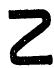
\includegraphics[keepaspectratio]{images/part002_bec1605a.jpg}}

In general, even in a Polish space, the complement of a Souslin subspace is not necessarily Souslin (cf.~Exercise 6); see, however, no. 6, Theorem 2, Corollary.

PROPOSITION 9. Let X be a metrizable space, and let A be a relatively compact Souslin subspace of X. Then there exists a compact metrizable space K, a decreasing sequence \((\mathbf{B}_{n})\) of subsets of K, each of which is a countable union of compact sets, and a continuous mapping \(f: K \to X\) , such that \(A = f\left(\bigcap_{n} B_{n}\right)\) .

Replacing X by \(\overline{\mathbf{A}}\) if necessary, we may suppose that X is compact and that A is dense in X. Since A is a Souslin space, there is a Polish space P and a continuous mapping \(g: \mathrm{P} \to \mathrm{X}\) such that \(g(\mathrm{P}) = \mathrm{A}\) . By no. 1, Theorem 1, Corollary 1, we may assume that P is the intersection of a decreasing sequence \((\mathbf{U}_n)\) of open subsets of the cube \(\mathbf{I}^{\mathbf{N}}\) . Let K be the space \(\mathbf{I}^{\mathbf{N}} \times \mathbf{X}\) , which is compact and metrizable (§ 2, no. 4, Theorem 1, Corollary 2). Let \(\mathbf{G} \subset \mathbf{P} \times \mathbf{X}\) be the graph of \(g\) , let \(\overline{\mathbf{G}}\) be the closure of G in K, and let \(f\) denote the projection of \(\mathbf{K} = \mathbf{I}^{\mathbf{N}} \times \mathbf{X}\) onto X; then clearly we have \(f(\mathbf{G}) = \mathbf{A}\) . Since \(g\) is continuous, G is closed in \(\mathbf{P} \times \mathbf{X}\) (Chapter I, § 8, no. 1, Proposition 2, Corollary 2) and \(\mathbf{G} = \overline{\mathbf{G}} \cap (\mathbf{P} \times \mathbf{X})\) ; hence \(\mathbf{G} = \bigcap_{n=1}^{n} \mathbf{B}_n\) , where

\[
\mathbf {B} _ {n} = \overline {{\mathbf {G}}} \cap (\mathbf {U} _ {n} \times \mathbf {X}).
\]

Since each \(U_{n}\) is a countable union of closed sets in \(I^{N}\) (§ 2, no. 5, Proposition 7), each \(B_{n}\) is a countable union of compact sets and the proof is complete.

\subsection{BOREL SETS}

DEFINITION 3. Let X be a set and let \(\mathfrak{X}\) be a set of subsets of X. \(\mathfrak{X}\) is said to be a \(\sigma\) -algebra on X if the following conditions are satisfied:

\begin{enumerate}
\def\labelenumi{\alph{enumi})}
\item
  The complement of every set of \(\mathfrak{S}\) belongs to \(\mathfrak{S}\) .
\item
  Every countable intersection of sets of \(\mathfrak{X}\) belongs to \(\mathfrak{X}\) .
\end{enumerate}

If \(\mathfrak{X}\) is a \(\sigma\) -algebra on \(\mathbf{X}\) , every countable union of sets of \(\mathfrak{X}\) belongs to \(\mathfrak{X}\) (for the complement of this union is an intersection of sets of \(\mathfrak{X}\) ).

The set \(\mathfrak{P}(\mathbf{X})\) of all subsets of X is clearly a \(\sigma\) -algebra. Every intersection of \(\sigma\) -algebras on X is a \(\sigma\) -algebra on X. For any subset of \(\mathfrak{P}(\mathbf{X})\) , there is therefore a smallest \(\sigma\) -algebra containing F; it is called the \(\sigma\) -algebra generated by F.

DEFINITION 4. In a topological space X, the elements of the \(\sigma\) -algebra generated by the set of all closed subsets of X are called Borel sets in X.

PROPOSITION 10. Let \(f\) be a continuous mapping of a topological space \(\mathbf{X}\) into a topological space \(\mathbf{Y}\) . Then the inverse image under \(f\) of every Borel set in \(\mathbf{Y}\) is a Borel set in \(\mathbf{X}\) .

Let \(\mathfrak{X}\) be the set of all subsets \(\mathbf{A}\) of \(\mathbf{Y}\) such that \(\overline{f}^1 (\mathbf{A})\) is a Borel set in \(\mathbf{X}\) . It follows immediately that \(\mathfrak{X}\) is a \(\sigma\) -algebra which contains all the closed subsets of \(\mathbf{Y}\) ; hence \(\mathfrak{X}\) contains all Borel sets in \(\mathbf{Y}\) .

PROPOSITION II. In a Souslin space X, every Borel set is a Souslin set.

Let \(\mathfrak{X}\) be the set of all subsets A of X such that both A and CA are Souslin sets. By Proposition 8 of no. 2, \(\mathfrak{X}\) is a \(\sigma\) -algebra. Every closed subset F of X belongs to \(\mathfrak{X}\) , for both F and CF are Souslin sets (no. 2, Proposition 5); hence \(\mathfrak{X}\) contains all Borel sets of X (cf.~no. 6, Theorem 2, Corollary).

COROLLARY. Let \(f\) be a continuous mapping of a Souslin space \(\mathbf{X}\) into a metrizable space \(\mathbf{Y}\) . If \(\mathbf{B}\) is any Borel set in \(\mathbf{X}\) , then \(f(\mathbf{B})\) is a Souslin set in \(\mathbf{Y}\) .

For B is a Souslin space, hence so is \(f(\mathbf{B})\) by the remark following Definition 2 (no. 2).

\pandocbounded{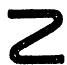
\includegraphics[keepaspectratio]{images/part002_bde2d1b5.jpg}}

Remarks. 1) Even when X and Y are Polish spaces it is not in general true that the image of a Borel set in X under a continuous mapping of X into Y is a Borel set in Y (cf.~Exercise 6; and no. 7, Theorem 3 Corollary).

\begin{enumerate}
\def\labelenumi{\arabic{enumi})}
\setcounter{enumi}{1}
\tightlist
\item
  Let X be a topological space and let Y be a Borel subset of X. Then the Borel sets of the space Y are exactly the Borel sets of X which are contained in Y. For (i) the Borel sets in X which are contained in Y form a σ-algebra on Y which contains the closed sets in Y and hence contains all Borel sets of Y; (ii) the subsets A of X such that A∩Y is a Borel set of Y form a σ-algebra on X which contains all the closed sets of X and therefore contains all Borel sets of X.
\end{enumerate}

\subsection{ZERO-DIMENSIONAL SPACES AND LUSIN SPACES}

DEFINITION 5. A topological space is said to be zero-dimensional if it is Hausdorff and if every point has a fundamental system of neighbourhoods which are both open and closed.

Every zero-dimensional space X is totally disconnected; for the component of a point x is contained in all the sets containing x which are both open and closed (Chapter I, § 11, no. 5), and the intersection of these sets is just \(\{x\}\) if \(\mathbf{X}\) is zero-dimensional.

Conversely, a locally compact totally disconnected space is zero-dimensional (Chapter II, § 4, no. 4, Proposition 6); but there exist totally disconnected metrizable spaces which are not zero-dimensional {[}Exercise 3 b){]}.

Every subspace of a zero-dimensional space is zero-dimensional, and topological sums and products of zero-dimensional spaces are zero-dimensional.

DEFINITION 6. A topological space X is a Lusin space if it is metrizable and if there exists a zero-dimensional Polish space P and a continuous bijective mapping of P onto X.

Every Lusin space is clearly a Souslin space.

PROPOSITION 12. A metrizable space is a Lusin space if and only if it is the image of a Polish space under a continuous bijective mapping.

The condition is clearly necessary; let us show that it is also sufficient. If f is a continuous bijection of a Lusin space X onto a metrizable space Y, it follows from Definition 6 that Y is a Lusin space. Hence we need only show that a Polish space is a Lusin space.

Notice first that, if X is a Lusin space, every closed (resp. open) subspace A of X is a Lusin space (cf.~no. 7, Theorem 3); for if f is a continuous bijection of a zero-dimensional Polish space P onto X, then \(\overline{f}^{1}(A)\) is closed (resp. open) in P and is therefore a zero-dimensional Polish subspace of P (no. 1, Propositions 1 and 2).

Every countable product of Lusin spaces is a Lusin space; this follows from Proposition 1 of no. 1 and the fact that every product of zero-dimensional spaces is zero-dimensional. Every countable intersection of Lusin subspaces of a Hausdorff topological space is a Lusin subspace; this follows from the preceding remarks and from Lemma 1 of no. 1. Furthermore:

LEMMA 2. If a metrizable space X is such that there exists a countable partition \((\mathbf{A}_{n})\) of X formed of Lusin subspaces, then X is a Lusin space.

For each n, let \(P_{n}\) be a zero-dimensional Polish space and let \(f_{n}\) be a continuous bijection of \(P_{n}\) onto \(A_{n}\) . If P is the topological sum of the \(P_{n}\) , then P is Polish (no. 1, Proposition 1) and zero-dimensional, and the mapping \(f: P \to X\) which agrees with \(f_{n}\) on \(P_{n}\) for each n is a continuous bijection of P onto X; hence the result.

Let us now show that the interval \(I = [0, i]\) of R is a Lusin space. Let J be the subspace of I consisting of all irrational numbers; then J is Polish (no. 1, Corollary to Proposition 3); also J is zero-dimensional, for if x is any point of J, the traces on J of intervals of R of the form {]}r, s{[}, where r and s are rational and r \textless{} x \textless{} s, form a fundamental system of open and closed neighbourhoods of x in J (because the traces on J of {]}r, s{[} and {[}r, s{]} are the same). Hence J is a Lusin subspace of I. Now J and the subspaces of I which consist each of a single rational point form a countable partition of I, and therefore I is a Lusin space by Lemma 2.

Let P be an arbitrary Polish space. By Corollary 1 to Theorem 1 (no. 1), P is homeomorphic to a subspace of the cube IN which is a countable intersection of open sets in IN. Since I is a Lusin space, the remarks at the beginning of the proof show that P is a Lusin space, and the proof of Proposition 12 is therefore complete.

\subsection{SIEVES}

DEFINITION 7. A sieve is a sequence \(\mathbf{C} = (\mathbf{C}_n, p_n)_{n \geqslant 0}\) such that, for each \(n\) , \(\mathbf{C}_n\) is a countable set and \(p_n\) is a surjection of \(\mathbf{C}_{n+1}\) onto \(\mathbf{C}_n\) .

For each pair of integers \(m, n\) such that \(0 \leqslant m \leqslant n\) , let \(p_{mn}\) denote the identity mapping of \(C_m\) onto itself if \(m = n\) , and the surjection \(p_m \circ p_{m+1} \circ \cdots \circ p_{n-1}\) of \(C_n\) onto \(C_m\) if \(m < n\) . Clearly \(p_{mq} = p_{mn} \circ p_{ng}\) whenever \(m \leqslant n \leqslant q\) , and we may therefore consider the inverse limit \(L(C)\) of the family \((C_n)\) with respect to the family of mappings \((p_{mn})\) (Set Theory, Chapter III, § 7). If each \(C_n\) is endowed with the discrete topology, then \(L(C)\) is an inverse limit of topological spaces (Chapter I, § 4, no. 4); as such, \(L(C)\) is called the topological space associated with the sieve \(C\) . \(L(C)\) is a closed subspace of the topological product \(\prod_n C_n\) , and it follows immediately that \(L(C)\) is a zero-dimensional Polish space (no. 4).

A sifting of a metric space X consists of a sieve \(\mathbf{C} = (\mathbf{C}_{n}, p_{n})\) and for each integer \(n \geqslant 0\) a mapping \(\varphi_{n}\) of \(C_{n}\) into the set of non-empty closed subsets of X of diameter \(\leqslant 2^{-n}\) , such that:

\begin{enumerate}
\def\labelenumi{\alph{enumi})}
\item
  X is the union of the sets \(\varphi_0(c)\) as \(c\) runs through \(\mathbf{C}_0\) ;
\item
  for each \(n\) and each \(c \in \mathbf{C}_n\) , \(\varphi_n(c)\) is the union of the sets \(\varphi_{n+1}(c')\) , where \(c'\) runs through \(\overline{\pmb{p}}_n(c)\) .
\end{enumerate}

A sifting is said to be strict if in addition, for each n, the sets \(\varphi_{n}(c)\) , as c runs through \(C_{n}\) , are mutually disjoint.

LEMMA 3. Every metric space X of countable type possesses a sifting. If also X is zero-dimensional, then X has a strict sifting.

Note first that if Y is a metric space of countable type and if \(\varepsilon\) is a real number \textgreater0, then there is a countable covering of Y by sets of diameter \(\leqslant\varepsilon\) (§2, no. 8, Proposition 13). If, moreover, Y is zero-dimensional, there is such a covering \((\mathbf{V}_{n})\) formed of sets which are both open and closed; if \(W_{n}\) is the intersection of \(V_{n}\) and \(\bigcap_{k<n}(\mathbf{Y}-\mathbf{V}_{k})\) , we see that the \(W_{n}\) are closed, of diameter \(\leqslant\varepsilon\) , pairwise disjoint and cover X. In any case, the closures of the non-empty sets of the covering form a countable covering of Y whose elements are non-empty closed sets of diameter \(\leqslant\varepsilon\) .

Let X be a metric space of countable type. Let \(C_{0}\) be the set of indices of a countable covering of X formed of non-empty closed sets of diameter \(\leqslant I\) , which are pairwise disjoint if X is zero-dimensional; \(\varphi_{0}\) shall be the mapping which associates with each index \(c \in C_{0}\) the corresponding set of the covering. Suppose that we have already defined the \(C_{i}\) and the \(\varphi_{i}\) and the surjective mappings \(p_{i}: C_{i+1} \to C_{i}\) for \(i \leqslant n\) in such a way that condition b) is satisfied for these indices. If \(c \in C_{n}\) , the space \(\varphi_{n}(c)\) has a countable covering by non-empty closed sets of diameter \(\leqslant I/2^{n+1}\) , which are mutually disjoint if X {[}and therefore \(\varphi_{n}(c)\) {]} is zero-dimensional; if \(\mathrm{I}(c)\) denotes the index set of this covering, we take \(c_{n+1}\) to be the sum of the sets \(\mathrm{I}(c)\) as c runs through \(C_{n}\) ; for each \(c' \in C_{n+1}\) , let \(p_{n}(c')\) denote the element \(c \in C_{n}\) such that \(c' \in \mathrm{I}(c)\) , and let \(\varphi_{n+1}(c')\) denote the set with index \(c'\) in the covering of \(\varphi_{n}(c)\) under consideration. Clearly we thus define by induction a sifting of X, and this sifting is strict if X is zero-dimensional; hence Lemma 3.

Now suppose that X is a complete metric space of countable type, and consider a sifting of X by a sieve C and mappings \(\varphi_{n}\) . If \(\gamma = (c_{n})\) is a point of the space \(\mathrm{L}(\mathrm{C})\) associated with C, the sequence \((\varphi_{n}(c_{n}))\) is a decreasing sequence of closed sets in X whose diameters tend to o; the intersection of this sequence of sets consists therefore of a single point, which we denote by \(f(\gamma)\) . Thus we have defined a mapping \(f: \mathrm{L}(\mathrm{C}) \to \mathrm{X}\) . If two points \(\gamma, \gamma'\) of \(\mathrm{L}(\mathrm{C})\) have the same i-th coordinates for \(i \leqslant n\) , it is clear that the distance between \(f(\gamma)\) and \(f(\gamma')\) is \(\leqslant 1/2^{n}\) , and therefore f is continuous, by virtue of the definition of the topology of \(\mathrm{L}(\mathrm{C})\) . For each \(x \in X\) it follows from the definition of a sifting that we can define by induction on n a sequence \(\gamma = (c_{n})\) such that \(x \in \varphi_{n}(c_{n})\) for each \(n \geqslant 0\) , and \(c_{n} = p_{n}(c_{n+1})\) ; hence \(x = f(\gamma)\) and so f is surjective. Furthermore, if the sifting is strict, the sequence \(\gamma = (c_{n})\) such that \(x = f(\gamma)\) is unique, and so in this case f is bijective. f is said to be the mapping induced by the sifting considered.

PROPOSITION 13. If X is any Lusin (resp. Souslin) space, there exists a sieve C and a continuous bijection (resp. surjection) of L(C) onto X.

Referring to the definition of a Lusin space (no. 4, Definition 6) {[}resp. a Souslin space (no. 2, Definition 2){]}, we reduce to the case where

X is Polish and zero-dimensional (resp. Polish), and the preceding argument then proves the result.

\subsection{SEPARATION OF SOUSLIN SETS}

THEOREM 2. Let X be a metrizable space. If we are given a sequence \((\mathbf{X}_{n})\) of mutually disjoint Souslin subspaces of X, then there exists a sequence \((\mathbf{B}_{n})\) of mutually disjoint Borel sets in X such that \(X_{n} \subset B_{n}\) for each n.

The proof rests on two lemmas :

LEMMA 4. Let \((\mathbf{A}_n), (\mathbf{A}_m')\) be two sequences of subsets of a topological space \(\mathbf{X}\) . Suppose that for each pair \((\mathbf{A}_n, \mathbf{A}_m')\) there is a Borel set \(\mathbf{B}_{nm}\) of \(\mathbf{X}\) such that \(\mathbf{B}_{nm} \supset \mathbf{A}_n\) and \(\mathbf{B}_{nm} \cap \mathbf{A}_m' = \emptyset\) . Then there is a Borel set \(\mathbf{B}\) of \(\mathbf{X}\) which contains \(\bigcup_{n} \mathbf{A}_n\) and does not meet \(\bigcup_{m} \mathbf{A}_m'\) .

For the Borel set \(\mathbf{B} = \bigcup_{n}\left(\bigcap_{m}\mathrm{B}_{nm}\right)\) satisfies these conditions.

LEMMA 5. Let X be a Hausdorff space and let A, A' be two disjoint Souslin subspaces of X. Then there is a Borel set B of X such that B ⊃ A and B ∩ A' = ∅.

By Proposition 13 of no. 5 there exist two sieves \(\mathbf{C}\) , \(\mathbf{C}'\) and continuous mappings \(f\) of \(\mathbf{L}(\mathbf{C})\) onto \(\mathbf{A}\) , \(f'\) of \(\mathbf{L}(\mathbf{C}')\) onto \(\mathbf{A}'\) , constructed by the method described in no. 5. For each \(n \geqslant 0\) and each \(c \in \mathbf{C}_n\) , let \(q_n(c)\) denote the subspace of \(\mathbf{L}(\mathbf{C})\) formed of all sequences \((c_k)_{k \geqslant 0}\) such that \(c_n = c\) ; \(q_n(c)\) is a closed subspace of \(\mathbf{L}(\mathbf{C})\) . For each \(\gamma = (c_n) \in \mathbf{L}(\mathbf{C})\) the sequence of closed sets \(q_n(c_n)\) is decreasing and forms a filter base with \(\gamma\) as limit. Moreover, for each \(c \in \mathbf{C}_n\) , the sets \(q_{n+1}(d)\) , where \(d\) runs through the set \(\overline{p_n}(c)\) in \(\mathbf{C}_{n+1}\) , form a partition of \(q_n(c)\) . Make the analogous definitions of notation for the sieve \(c'\) .

We shall argue by contradiction and assume that every Borel set which contains A meets \(A'\) . In the first place, it follows from Lemma 4 and the definition of a sifting that there exist \(c_{0} \in C_{0}\) and \(c_{0}' \in C_{0}'\) such that every Borel set containing \(f(q_{0}(c_{0}))\) meets \(f'(q_{0}'(c_{0}'))\) . We can then define, by induction on n,

\[
\gamma = (c _ {n}) \in \mathrm{L} (\mathrm{C}) \quad \text { and } \quad \gamma^ {\prime} = (c _ {n} ^ {\prime}) \in \mathrm{L} (\mathrm{C} ^ {\prime})
\]

as follows: suppose that \(c_i\) and \(c_i'\) have already been defined for \(i < n\) , in such a way that for each index \(i < n\) every Borel set containing \(f(q_i(c_i))\) meets \(f'(q_i'(c_i'))\) ; applying Lemma 4 and the definition of a sifting to the sets \(f(q_{n-1}(c_{n-1}))\) and \(f'(q_{n-1}'(c_{n-1}'))\) , we see that there exist \(c_n \in \mathbf{C}_n\) and \(c_n' \in \mathbf{C}_n'\) such that \(p_{n-1}(c_n) = c_{n-1}\) and \(p_{n-1}(c_n') = c_{n-1}'\) .

and such that every Borel set containing \(f(q_n(c_n))\) meets \(f'(q_n'(c_n'))\) . Now the sequence \(f(q_n(c_n))\) converges to a point \(a = f(\gamma) \in \mathbf{A}\) , and the sequence \(f'(q_n'(c_n'))\) converges to a point \(a' = f'(\gamma') \in \mathbf{A}'\) . Since \(\mathbf{A} \cap \mathbf{A}' = \emptyset\) and \(\mathbf{X}\) is Hausdorff, there is a closed neighbourhood \(\mathbf{V}\) of \(a\) which does not contain \(a'\) , and thus for \(n\) sufficiently large, \(\mathbf{V}\) contains \(f(q_n(c_n))\) and does not meet \(f'(q_n'(c_n'))\) . This is a contradiction, since \(\mathbf{V}\) is a Borel set.

To prove Theorem 2, let \(\mathbf{Y}_n\) denote the union of the sets \(\mathbf{X}_i\) such that \(i \neq n\) ; then \(\mathbf{Y}_n\) is a Souslin subspace of \(\mathbf{X}\) (no. 2, Proposition 8). For each index \(n\) there exists a Borel set \(\mathbf{B}_n'\) which contains \(\mathbf{X}_n\) and does not meet \(\mathbf{Y}_n\) , by Lemma 5. Let \(\mathbf{B}_n\) be the intersection of \(\mathbf{B}_n'\) and \(\bigcap_{i < n} (\mathbf{X} - \mathbf{B}_i')\) . Then the \(\mathbf{B}_n\) are Borel sets, are mutually disjoint, and are such that \(\mathbf{B}_n \supset \mathbf{X}_n\) for each \(n\) .

COROLLARY. If a countable partition of a metrizable space is formed of Souslin sets, then these sets are Borel sets. In particular, every Souslin set in a metrizable space, whose complement is a Souslin set, is a Borel set.

\subsection{LUSIN SPACES AND BOREL SETS}

THEOREM 3. Let X be a Lusin space. Then a subspace of X is a Lusin space if and only if it is a Borel set.

This theorem is a consequence of the following two lemmas :

LEMMA 6. In a Lusin space X, every Borel set is a Lusin subspace of X.

Let \(\mathfrak{X}\) be the set of all subsets A of X such that both A and \(\complement A\) are Lusin subspaces of X. Since every closed set and every open set in X is a Lusin subspace of X (no. 4), \(\mathfrak{X}\) contains all closed subsets of X, and the lemma will therefore be proved if we can show that \(\mathfrak{X}\) is a \(\sigma\) -algebra on X. For this it is enough to show that if \((A_n)\) is a sequence of sets of \(\mathfrak{X}\) , then \(\bigcap_{n} A_n\) and \(\bigcup_{n} A_n\) are Lusin subspaces of X. Now we have seen in no. 4 that every countable intersection of Lusin subspaces is a Lusin subspace. On the other hand, if \(B_n\) is the intersection of \(A_n\) and \(\bigcap_{i < n} \complement A_i\) , it follows from the hypothesis and the preceding remark that \(B_n\) is a Lusin subspace; and since \(\bigcup_{n} A_n = \bigcup_{n} B_n\) , the subspace \(\bigcup_{n} A_n\) is a Lusin subspace by Lemma 2 of no. 4.

LEMMA 7. Every Lusin subspace A of a metrizable space X is a Borel set in X.

By Proposition 13 of no. 5 there exist a sieve C and a continuous bijection \(f\) of \(\mathbf{L}(\mathbf{C})\) onto A. With the notation of Lemma 5 of no. 6, for each integer \(n\) and each \(c \in \mathbf{C}_n\) , let \(g_n(c)\) denote the subspace \(f(q_n(c))\) of X; it is a Lusin subspace and therefore a Souslin subspace of X. As \(c\) runs through \(\mathbf{C}_n\) , the sets \(g_n(c)\) are pairwise disjoint, because \(f\) is bijective; hence, by Theorem 2 of no. 6, there is a family \(c \to g_n'(c) (c \in \mathbf{C}_n)\) of Borel sets in X, pairwise disjoint and such that \(g_n'(c) \supset g_n(c)\) for all \(c \in \mathbf{C}_n\) . Replacing \(g_n'(c)\) by its intersection with the closure \(\overline{g_n(c)}\) of \(g_n(c)\) in X if necessary, we may suppose that \(g_n'(c) \subset \overline{g_n(c)}\) . Let \(c_{n-1}, c_{n-2}, \ldots, c_0\) denote the images of \(c\) in \(\mathbf{C}_{n-1}, \mathbf{C}_{n-2}, \ldots, \mathbf{C}_0\) , under the surjections

\[
p _ {n - 1, n} = p _ {n - 1}, p _ {n - 2, n} = p _ {n - 2} \circ p _ {n - 1}, \dots , p _ {0 n} = p _ {0} \circ p _ {1} \circ \dots \circ p _ {n - 1}
\]

respectively; and let \(h_n(c)\) denote the intersection of the sets

\[
g _ {n} ^ {\prime} (c), g _ {n - 1} ^ {\prime} \left(c _ {n - 1}\right), \dots , g _ {o} ^ {\prime} \left(c _ {0}\right).
\]

Since \(q_{i}(c_{i}) \supset q_{n}(c)\) for \(0 \leqslant i \leqslant n - 1\) , \(h_{n}(c)\) contains \(g_{n}(c)\) ; it is clear also that \(h_{n}(c)\) is a Borel set and is contained in \(g_{n}(c)\) , and that as \(c\) runs through \(\mathbf{C}_{n}\) , the \(h_{n}(c)\) are mutually disjoint sets; finally, by construction, for each \(c' \in \mathbf{C}_{n+1}\) we have \(h_{n+1}(c') \subset h_n(p_n(c'))\) . Let then \(\mathbf{B}_n\) be the union of the sets \(h_n(c)\) as \(c\) runs through \(\mathbf{C}_n\) ; \(\mathbf{B}_n\) is a Borel set, and \(\mathbf{B}_{n+1} \subset \mathbf{B}_n\) ; also \(\mathbf{B}_n\) contains the union of the sets \(g_n(c) (c \in \mathbf{C}_n)\) , which is A. Let B be the intersection of the decreasing sequence of sets \(\mathbf{B}_n\) ; B is a Borel set and contains A. We shall show that B = A, and this will complete the proof.

Let \(x\) be a point of \(\mathbf{B}\) . Then, for each integer \(n\) , there exists a unique \(c \in \mathbf{C}_n\) such that \(x \in h_n(c)\) ; let us denote this \(c\) by \(c_n(x)\) . The sequence \((c_n(x))_{n \geqslant 0}\) belongs to \(\mathbf{L}(\mathbf{C})\) . The decreasing sequence \((g_n(c_n(x)))\) converges by definition to a point \(a \in \mathbf{A}\) ; the sequence of closures of these sets also converges to \(a\) in \(\mathbf{X}\) , hence a fortiori so does the sequence \((h_n(c_n(x)))\) . Now \(x\) belongs to all the sets \(h_n(c_n(x))\) , therefore \(x = a \in \mathbf{A}\) . Lemma 7 is thus proved, and with it Theorem 3.

COROLLARY. If \(f\) is a continuous injective mapping of a Lusin space (or, in particular, a Polish space) \(\mathbf{X}\) into a metrizable space \(\mathbf{Y}\) , then \(f(\mathbf{X})\) is a Borel set in \(\mathbf{Y}\) .

\subsection{BOREL SECTIONS}

THEOREM 4. Let X be a Polish space and let R be an equivalence relation on X, such that the equivalence classes mod R are closed in X and the saturation (with respect to R) of each closed set in X is a Borel set. Then there is a Borel set in X which meets each equivalence class in exactly one point.

Consider a metric on X compatible with its topology, and with respect to which X is complete. By Lemma 3 of no. 5, there exists a sifting of X, defined by a sieve \(\mathbf{C} = (\mathbf{C}_{n}, p_{n})\) and a sequence of mappings \((\varphi_{n})\) . For each \(c \in C_{n}\) , let \(g_{n}(c)\) be the saturation of the closed set \(\varphi_{n}(c)\) with respect to R; by hypothesis, \(g_{n}(c)\) is a Borel set in X.

Since each set \(\mathbf{C}_n\) is countable, we can linearly order each \(\mathbf{C}_n\) in such a way that the set of elements smaller than a given element is finite. For each \(c \in \mathbf{C}_n\) we define a set \(h_n(c)\) by induction on \(n\) , as follows. In the first place, for \(c \in \mathbf{C}_0\) , \(h_0(c)\) is the intersection of \(\varphi_0(c)\) and the sets \(\mathbf{X} - g_0(c')\) , where \(c' \in \mathbf{C}_0\) and \(c' < c\) . For \(c \in \mathbf{C}_{n+1}\) , \(h_{n+1}(c)\) is the intersection of \(\varphi_{n+1}(c)\) , \(h_n(\mathbf{P}_n(c))\) and the sets \(\mathbf{X} - g_{n+1}(c')\) for \(c' \in \mathbf{C}_{n+1}\) , \(p_n(c') = p_n(c)\) and \(c' < c\) . The \(h_n(c)\) are clearly Borel sets.

We shall prove the following assertion: for each integer \(n \geqslant 0\) and each equivalence class \(\mathbf{H} \mod \mathbb{R}\) , there is a unique element \(c \in \mathbf{C}_n\) such that \(h_n(c)\) meets \(\mathbf{H}\) , and we have

\[
h (c _ {n}) \cap \mathrm{H} = \varphi_ {n} (c) \cap \mathrm{H},
\]

which is therefore a closed set. For \(n = 0\) , consider the smallest element \(c \in \mathbf{C}_0\) such that \(\varphi_0(c)\) meets \(\mathbf{H}\) ; then \(\varphi_0(c) \cap \mathbf{H}\) does not meet any set \(g_0(c')\) for which \(c' \in \mathbf{C}_0\) and \(c' < c\) ; hence it is contained in \(h_0(c) \cap \mathbf{H}\) and consequently is equal to this set; moreover, we have \(\mathbf{H} \subset g_0(c)\) and therefore \(h_0(c') \cap \mathbf{H}\) is empty for \(c' \in \mathbf{C}_0\) and \(c' > c\) ; thus the assertion is proved for \(n = 0\) . We continue by induction on \(n\) : if there exists \(c \in \mathbf{C}_{n+1}\) such that \(h_{n+1}(c)\) meets \(\mathbf{H}\) , then it follows from the relation \(h_{n+1}(c) \subset h_n(p_n(c))\) and the inductive hypothesis that \(p_n(c)\) is the unique element \(d \in \mathbf{C}_n\) such that \(h_n(d)\) meets \(\mathbf{H}\) . Observe that \(h_n(d)\) , which is contained in \(\varphi_n(d)\) , is contained in the union of the sets \(\varphi_n(c)\) for which \(c \in p_n(d)\) , by the definition of a sifting; there is therefore a smallest element \(c \in p_n(d)\) such that \(\varphi_{n+1}(c)\) meets \(\mathbf{H}\) . We have therefore

\[
\varphi_ {n + 1} (c) \cap \mathrm{H} \subset \varphi_ {n} (d) \cap \mathrm{H} = h _ {n} (d) \cap \mathrm{H}
\]

by the inductive hypothesis. Hence

\[
\varphi_ {n + 1} (c) \cap \mathrm{H} \subset \varphi_ {n + 1} (c) \cap h _ {n} (d),
\]

and since by definition \(\varphi_{n+1}(c) \cap \mathbf{H}\) meets none of the sets \(g_{n+1}(c')\) for which \(c' \in p_n(d)\) and \(c' < c\) , it follows from the definition of \(h_{n+1}(c)\) that \(\varphi_{n+1}(c) \cap \mathbf{H} = h_{n+1}(c) \cap \mathbf{H}\) . Moreover, we have \(\mathbf{H} \subset g_{n+1}(c)\) and therefore, if \(c' \in p_n(d)\) is such that \(c' > c\) , \(h_{n+1}(c') \cap \mathbf{H}\) is empty. Hence the assertion is proved for all \(n\) .

For each integer \(n\) , let \(\mathbf{S}_n\) be the union of the sets \(h_n(c)\) , where \(c\) runs through \(\mathbf{C}_n\) . The set \(\mathbf{S}_n\) is a Borel set, and we have \(\mathbf{S}_{n+1} \subset \mathbf{S}_n\) .

Let S be the intersection of the sets \(S_{n}\) , which is also a Borel set in X; we shall show that S meets each equivalence class H mod R in exactly one point. For each n, let \(c_{n}(H)\) be the unique element \(c \in C_{n}\) such that \(h_{n}(c)\) meets H; then \(\mathbf{S}_{n} \cap \mathbf{H} = \varphi_{n}(c_{n}(\mathbf{H})) \cap \mathbf{H}\) , and \(S \cap H\) is the intersection of the sets \(\varphi_{n}(c_{n}(\mathbf{H})) \cap \mathbf{H}\) . Since the sequence \((c_{n}(\mathbf{H}))\) belongs to L(C), the decreasing sequence of closed sets \(\varphi_{n}(c_{n}(\mathbf{H}))\) , whose diameter tends to o, converges to a point \(x \in X\) , since X is complete. The intersection of the closed sets \(\varphi_{n}(c_{n}(\mathbf{H})) \cap \mathbf{H}\) therefore consists of the point x alone, and the proof of Theorem 4 is complete.

Remark. In particular a closed equivalence relation R satisfies the hypotheses of Theorem 4. When X is a compact metrizable space, Theorem 4 therefore applies to any Hausdorff equivalence relation R, since a Hausdorff equivalence relation on a compact space is closed (Chapter I, § 10, no. 4, Proposition 8).

\subsection{CAPACITABILITY OF SOUSLIN SETS}

DEFINITION 8. Let X be a Hausdorff topological space. A capacity on X is a mapping f of the set \(\mathfrak{P}(\mathbf{X})\) of all subsets of X into the extended real line \(\overline{\mathbf{R}}\) , satisfying the following conditions:

\((\mathbf{CA}_{\mathbf{I}})\) If \(\mathbf{A} \subset \mathbf{B}\) , then \(f(\mathbf{A}) \leqslant f(\mathbf{B})\) .

\((\mathbf{CA}_{\mathbf{II}})\) If \((\mathbf{A}_n)\) is any increasing sequence of subsets of \(\mathbf{X}\) , then

\[
f \left(\bigcup_ {n} \mathrm{A} _ {n}\right) = \sup _ {n} f (\mathrm{A} _ {n}).
\]

\((\mathbf{CA}_{\mathbf{III}})\) If \((\mathbf{K}_n)\) is any decreasing sequence of compact subsets of \(\mathbf{X}\) , then

\[
f \left(\bigcap_ {n} \mathrm{K} _ {n}\right) = \inf _ {n} f (\mathrm{K} _ {n}).
\]

Examples. * Let \(\mu\) be a positive measure on a locally compact space X; then the corresponding outer measure \(\mu^{*}\) is a capacity on X. It can be shown that in Euclidean space \(\mathbf{R}^{n}\) ( \(n \geqslant 3\) ), the ``Newtonian outer capacity'' is a capacity in the sense of Definition 8. *

DEFINITION 9. Let \(f\) be a capacity on \(\mathbf{X}\) ; a subset \(\mathbf{A}\) of \(\mathbf{X}\) is said to be capacitable (with respect to \(f\) ) if \(f(\mathbf{A}) = \sup_k f(\mathbf{K})\) , where \(\mathbf{K}\) runs through the set of compact subsets of \(\mathbf{A}\) .

* For example, if \(f\) is an outer measure \(\mu^{*}\) , every open set is capacitable; the capacitable sets A such that \(\mu^{*}(A) < +\infty\) are precisely the \(\mu\) -integrable sets. *

PROPOSITION 14. Let K be a compact space and let f be a capacity on K. If A is the intersection of a decreasing sequence \((\mathbf{A}_{n})\) of subsets of K, each of which is a countable union of closed sets, then A is capacitable.

It is enough to show that, for each \(a < f(A)\) , there is a closed set \(\mathbf{C} \subset \mathbf{A}\) such that \(f(\mathbf{C}) \geqslant a\) . Let us first show that there exists a sequence \((\mathbf{B}_n)_{n \geqslant 1}\) of closed sets such that \(\mathbf{B}_n \subset \mathbf{A}_n\) and such that, if we define a sequence \((\mathbf{C}_n)\) inductively by the conditions \(\mathbf{C}_0 = \mathbf{A}\) , \(\mathbf{C}_n = \mathbf{C}_{n-1} \cap \mathbf{B}_n\) for \(n \geqslant 1\) , then \(f(\mathbf{C}_n) > a\) for each \(n \geqslant 0\) . Suppose the \(\mathbf{B}_i\) have been defined for \(i < n\) ; by hypothesis we have \(\mathbf{C}_{n-1} \subset \mathbf{A} \subset \mathbf{A}_n\) and \(f(\mathbf{C}_{n-1}) > a\) ; since \(\mathbf{A}_n\) is the union of an increasing sequence of closed sets \(\mathbf{D}_j\) , it follows from \((\mathbf{CA}_{\mathbf{II}})\) that

\[
f \left(\mathrm{C} _ {n - 1}\right) = \sup _ {j} f \left(\mathrm{C} _ {n - 1} \cap \mathrm{D} _ {j}\right).
\]

Hence there is an index \(j\) such that \(f(\mathbf{C}_{n-1} \cap \mathbf{D}_j) > a\) , and we may take \(\mathbf{B}_n = \mathbf{D}_j\) .

Now let \(\mathbf{C} = \bigcap_{n}\mathbf{C}_{n}\) . Since \(\mathbf{A} = \bigcap_{n}\mathbf{A}_{n}\) and \(\mathbf{B}_n\subset \mathbf{A}_n\) we have

\[
\mathrm{C} = \bigcap_ {n} \mathrm{B} _ {n};
\]

the set C is therefore compact and contained in A.

Let \(B_n' = B_1 \cap B_2 \cap \cdots \cap B_n\) ; \((B_n')\) is a decreasing sequence of compact subsets of K; as \(C_n \subset C_i \subset B_i\) for i \textless{} n we also have \(C_n \subset B_n'\) . By \((CA_{III})\) , \(f(C) = \inf_{n} f(B_n')\) , and since \(C \subset C_n \subset B_n'\) we also have \(f(C) = \inf_{n} f(C_n) \geqslant a\) . This completes the proof.

THEOREM 5. Let X be a metrizable space and let Y be a relatively compact Souslin subspace of X. Then Y is capacitable with respect to every capacity f on X.

We have seen (no. 2, Proposition 9) that there exists a compact space K, a decreasing sequence \((\mathbf{A}_{n})\) of subsets of K, each of which is a countable union of compact sets, and a continuous mapping \(\varphi: K \to X\) such that \(Y = \varphi\left(\bigcap_{n} A_{n}\right)\) . By Proposition 14, \(\bigcap_{n} A_{n}\) is capacitable with respect to every capacity on K. Theorem 5 is therefore a consequence of the following proposition:

PROPOSITION 15. Let \(\varphi\) be a continuous mapping of a Hausdorff space K into a Hausdorff space X, and let \(f\) be a capacity on X. If for each subset A of K we put \(g(A) = f(\varphi(A))\) , then \(g\) is a capacity on K; moreover, if A is capacitable with respect to \(g\) , then \(\varphi(A)\) is capacitable with respect to \(f\) .

It is clear that \(g\) satisfies axioms \((\mathbf{CA}_{\mathbf{I}})\) and \((\mathbf{CA}_{\mathbf{II}})\) . On the other hand, let \((\mathbf{C}_n)\) be a decreasing sequence of compact subsets of \(\mathbf{K}\) , and let \(\mathbf{C} = \bigcap_{n} \mathbf{C}_n\) ; the sets \(\varphi(\mathbf{C})\) are compact, and their intersection is \(\varphi(\mathbf{C})\) ; for this intersection certainly contains \(\varphi(\mathbf{C})\) , and if \(x \in \varphi(\mathbf{C}_n)\) for all \(n\) , then the sets \(\overline{\varphi}^1(x) \cap \mathbf{C}_n\) form a decreasing sequence of non-empty compact subsets of \(\mathbf{K}\) , and therefore their intersection is not empty. We have therefore \(f(\varphi(\mathbf{C})) = \inf_{n} f(\varphi(\mathbf{C}_n))\) , that is \(g(\mathbf{C}) = \inf_{n} g(\mathbf{C}_n)\) ; thus \(g\) satisfies axiom \((\mathbf{CA}_{\mathbf{III}})\) and is therefore a capacity on \(\mathbf{K}\) .

Now let A be a subset of K which is capacitable with respect to g; if \(a < f(\varphi(A)) = g(A)\) , then there is a compact set \(C \subset A\) such that \(g(C) \geqslant a\) ; thus \(\varphi(C)\) is a compact set contained in \(\varphi(A)\) , and \(f(\varphi(C)) \geqslant a\) . This shows that \(\varphi(A)\) is capacitable with respect to f, and completes the proof of Proposition 15 and hence of Theorem 5.

Remark. * If \(\mu\) is a positive measure on a locally compact metrizable space X, then every Souslin subset A of X is \(\mu\) -measurable. For if K is any compact subset of X, K∩A is a relatively compact Souslin set, hence is capacitable with respect to \(\mu^{*}\) and consequently \(\mu\) -integrable. Note that the complement in X of a Souslin set, although not in general a Souslin set, is \(\mu\) -measurable *.

\appendix
\setcounter{chapter}{9}
\renewcommand{\thechapter}{\Roman{chapter}}
\setcounter{subsection}{0}
\renewcommand{\thesubsection}{\arabic{subsection}}

\section*{APPENDIX: INFINITE PRODUCTS IN NORMED ALGEBRAS}
\phantomsection
\addcontentsline{toc}{section}{Appendix: Infinite products in normed algebras}

\subsection{MULTIPLIABLE SEQUENCES IN A NORMED ALGEBRA}

Let A be a normed algebra over a non-discrete valued field K (Chapter IX, § 3, no. 7, Definition 9); we shall denote by \(||x||\) the norm of an element \(x \in A\) , and we shall assume that this norm satisfies the inequality \(||xy|| \leqslant ||x|| \cdot ||y||\) ; also we shall assume that A has an identity element \(e\) . Let \((x_n)_{n \in \mathbb{N}}\) be an infinite sequence of points of A. Every finite subset J of N, linearly ordered by the ordering of N, defines a sequence \((x_n)_{n \in J}\) of points of A, and we define the product

\[
p _ {J} = \prod_ {n \in J} x _ {n}
\]

of this sequence; this product is called the finite partial product of the sequence \((\pmb{x}_n)_{n\in \mathbb{N}}\) , corresponding to the finite subset \(J\) of \(\mathbb{N}\) (recall that if \(J = \emptyset\) we put \(\prod_{n\in \emptyset}x_n = e\) ).

DEFINITION 1. The sequence \((\pmb{x}_n)_{n\in \mathbb{N}}\) is said to be multipliable in the normed algebra \(\mathbf{A}\) if the mapping \(\mathbf{J}\to \pmb{p}_{\mathbf{J}}\) has a limit with respect to the filter of sections of the set \(\mathfrak{F}(\mathbf{N})\) of finite subsets of \(\mathbf{N}\) , ordered by the relation \(c\) ; this limit is called the product of the sequence \((\pmb{x}_n)_{n\in \mathbb{N}}\) , and is denoted by \(\prod_{n\in \mathbb{N}}\pmb{x}_n\) (or simply \(\prod_{n}\pmb{x}_n\) ); the \(\pmb{x}_n\) are called the factors of this product.

Definition 1 is equivalent to the following: the sequence \((\pmb{x}_n)\) is multipliable and its product is \(\pmb{p}\) if for each \(\varepsilon > 0\) there exists a finite subset \(J_0\) of \(\mathbf{N}\) such that, for every finite subset \(J \supset J_0\) of \(\mathbf{N}\) , we have \(||\pmb{p}_{\mathrm{J}} - \pmb{p}|| \leqslant \varepsilon\) .

Remarks. 1) When A is a commutative algebra, Definition 1 is identical with that given in Chapter III, § 5, no. 1, Remark 3; but when A is not commutative, the order structure of the index set N is essentially involved in Definition 1. If \(\sigma\) is an arbitrary permutation of N, we cannot in general assert that the sequence \((\pmb{x}_{\sigma(n)})\) is multipliable if the sequence \((x_{n})\) is multipliable; and if both sequences are multipliable, their products will in general be different.

\begin{enumerate}
\def\labelenumi{\arabic{enumi})}
\setcounter{enumi}{1}
\tightlist
\item
  Definition 1 can be immediately generalized to the case of a family \((\pmb{x}_n)_{n\in I}\) whose index set I is a subset of \(\mathbf{Z}\) (linearly ordered by the order induced by that of \(\mathbf{Z}\) ). We leave it to the reader to extend to this case the results below (cf.~Exercises 1 and 2).
\end{enumerate}

\subsection{MULTIPLIABILITY CRITERIA}

From now on we shall assume that the normed algebra A is complete.

THEOREM 1. Let \((\pmb{x}_n)_{n\in \mathbb{N}}\) be a sequence of points in a complete normed algebra A. a) If \((\pmb{x}_n)\) is multipliable and if its product is a unit of A, then for each \(\varepsilon >0\) there exists a finite subset \(\mathbf{J}_0\) of N such that, for every finite subset L of N which does not meet \(\mathbf{J}_0\) , we have \(||e - p_{\mathrm{L}}||\leqslant \varepsilon\) .

\begin{enumerate}
\def\labelenumi{\alph{enumi})}
\setcounter{enumi}{1}
\item
  Conversely, if the sequence \((\pmb{x}_n)\) satisfies this condition, it is multipliable. Moreover, if each \(\pmb{x}_n\) is a unit, then \(\prod_{n\in \mathbb{N}}\pmb{x}_n\) is a unit.
\end{enumerate}

a) Let \(\pmb{p}\) be the product of the multipliable sequence \((\pmb{x}_n)\) , and suppose that \(\pmb{p}\) is a unit in A; then (Chapter IX, § 3, no. 7, Proposition 13) there exist \(\alpha > 0\) and \(a > 0\) such that, for all \(y \in A\) for which we have

\[
\left| \left| \boldsymbol {y} - \boldsymbol {p} \right| \right| \leqslant \alpha ,
\]

y is a unit and \(\|y^{-1}\|\leqslant a\) . By hypothesis, for every \(\varepsilon\) such that \(o<\varepsilon<\alpha\) , there is a finite subset \(H_{0}\) of N such that, for every finite subset H of N containing \(H_{0}\) , we have \(\|p_{H}-p\|\leqslant\varepsilon\) . Let \(J_{0}=[0,m]\) be an interval of N which contains \(H_{0}\) ; for each finite subset L of N which does not meet \(J_{0}\) , the integers belonging to L are all greater than those belonging to \(H_{0}\) ; hence, if \(H=H_{0}\cup L\) , we have \(p_{H}=p_{H_{0}}p_{L}\) . Now, since \(\|p_{H_{0}}-p\|\leqslant\varepsilon\leqslant\alpha\) , \(p_{H_{0}}\) is a unit, and

\[
\left| \left| e - p _ {\mathrm{H} _ {0}} ^ {- 1} p \right| \right| \leqslant \varepsilon \left| \left| p _ {\mathrm{H} _ {0}} ^ {- 1} p \right| \right| \leqslant a \varepsilon ;
\]

since \(||p_{\mathrm{H_0}}p_{\mathrm{L}} - p|| \leqslant \varepsilon\) , we deduce

\[
\left| \left| p _ {\mathrm{L}} - p _ {\mathrm{H} _ {0}} ^ {- 1} p \right| \right| \leqslant \varepsilon \left| \left| p _ {\mathrm{H} _ {0}} ^ {- 1} \right| \right| \leqslant a \varepsilon ,
\]

and finally \(||e - p_{\mathrm{L}}|| \leqslant 2a\varepsilon\) .

\begin{enumerate}
\def\labelenumi{\alph{enumi})}
\setcounter{enumi}{1}
\tightlist
\item
  Suppose that, for each \(\varepsilon > 0\) , there exists a finite subset \(J_0\) of \(\mathbf{N}\) such that, for every finite subset \(\mathbf{L}\) of \(\mathbf{N}\) which does not meet \(J_0\) , we have \(\|e - p_{\mathbf{L}}\| \leqslant \varepsilon\) . Let \(H_0 = [0, p]\) be an interval of \(\mathbf{N}\) which contains \(J_0\) ; then every finite subset \(\mathbf{H}\) of \(\mathbf{N}\) which contains \(H_0\) can be written in the form \(H_0 \cup L\) , where the integers in \(\mathbf{L}\) are all greater than those in \(H_0\) ; hence we have \(p_H = p_{H_0}p_L\) , and since \(\mathbf{L}\) does not meet \(J_0\) , \(||p_H - p_{H_0}|| \leqslant \varepsilon ||p_{H_0}||\) , and consequently \(||p_H|| = (1 + \varepsilon)||p_{H_0}||\) . If \(p_{H_0} = 0\) , the sequence \((x_n)\) is evidently multipliable and its product is 0; excluding this trivial case, there is an interval \(H_1 = [0, q]\) containing \(H_0\) and such that, for every finite subset L of N which does not meet \(H_1\) , we have \(||e - p_L|| \leqslant \varepsilon (||p_{H_0}||)^{-1}\) . As above, it follows that, for each finite subset \(H \supset H_1\) ,
\end{enumerate}

\[
\left| \left| p _ {\mathrm{H}} - p _ {\mathrm{H} _ {4}} \right| \right| \leqslant \left(\left| \left| p _ {\mathrm{H} _ {0}} \right| \right|\right) ^ {- 1} \left| \left| p _ {\mathrm{H} _ {4}} \right| \right| \varepsilon \leqslant \varepsilon (\mathrm{I} + \varepsilon).
\]

Cauchy's criterion therefore shows that \(J \to p_J\) has a limit in \(A\) with respect to the directed set \(\mathfrak{F}(N)\) .

If all the \(x_{n}\) are units, then so are all the finite partial products \(p_{J}\) ; hence for each finite subset H containing \(H_{0}\) we have

\[
\left| \left| e - p _ {\mathrm{H} _ {0}} ^ {- 1} p _ {\mathrm{H}} \right| \right| \leqslant \varepsilon ,
\]

and this shows that, in the multiplicative group G of units of A, the image under the mapping \(J \rightarrow p_{J}\) of the section filter of \(\mathfrak{F}(N)\) is a Cauchy filter base with respect to the left uniformity of G; but since G is complete (Chapter IX, § 3, no. 7, Proposition 13), the limit of the mapping \(J \rightarrow p_{J}\) belongs to G.

Remark. If \((\pmb{x}_n)\) is multipliable and its product is not a unit, the condition of Theorem 1 is not necessarily satisfied: for example, if all the \(x_n\) are equal to the same element \(x\) , where \(||x|| < 1\) , the sequence \((\pmb{x}_n)\) is multipliable and its product is 0, and for each non-empty finite subset H of N, we have \(\| p_{\mathbf{H}} \| \leqslant \| x \| < 1 \leqslant \| e \|\) .

COROLLARY I. If \((\pmb{x}_n)\) is a multipliable sequence whose product is a unit of A, then \(\lim_{n\to \infty}\pmb{x}_n = \pmb{e}\) .

COROLLARY 2. If \((\pmb{x}_n)\) is a multipliable sequence whose product is a unit of A, then every subsequence \((\pmb{x}_{n_k})_{k\in \mathbb{N}}\) of \((\pmb{x}_n)[(n_k)\) being a strictly increasing sequence of integers{]} is multipliable.

This follows immediately from the criterion of Theorem 1.

THEOREM 2. Let A be a complete normed algebra. If \((\pmb{u}_n)\) is an absolutely convergent series of elements of A, then the sequence \((\pmb{e} + \pmb{u}_n)\) is multipliable in A; and if all the elements \(\pmb{e} + \pmb{u}_n\) are units in A, then so is \(\prod_{n\in \mathbb{N}}(\pmb {e} + \pmb{u}_n)\) .

Let us apply the criterion of Theorem 1. For every finite subset L of N, we have \(p_{L} - e = \prod_{n \in L} (e + u_n) - e = \sum_{M} \left( \prod_{n \in M} u_n \right)\) , where M runs through the set of all non-empty subsets of L (linearly ordered by the induced ordering). Since \(\left\| \prod_{n\in \mathbf{M}}\pmb {u}_n\right\| \leqslant \prod_{n\in \mathbf{M}}||\pmb {u}_n||,\) we may write

\[
\left| \left| \boldsymbol {p} _ {\mathrm{L}} - \boldsymbol {e} \right| \right| \leqslant \sum_ {\mathbf {M}} \left(\prod_ {n \in \mathbf {M}} \left| \left| \boldsymbol {u} _ {n} \right|\right)\right) = \prod_ {n \in \mathbf {L}} (\mathrm{I} + \left| \left| \boldsymbol {u} _ {n} \right|\right) - \mathrm{I}.
\]

Now since the series whose general term is \(||\boldsymbol{u}_n||\) is convergent by hypothesis, the sequence \((\mathbf{I} + ||\boldsymbol{u}_n||)\) is multiplierable in \(\mathbf{R}_+^*\) (Chapter IV, § 7, no. 4, Theorem 4). Hence for each \(\varepsilon > 0\) there exists a finite subset \(J_0\) of \(\mathbf{N}\) such that, for every finite subset \(\mathbf{L}\) of \(\mathbf{N}\) which does not meet \(J_0\) , we have \(\left| \prod_{n \in \mathbf{L}} (\mathbf{I} + ||\boldsymbol{u}_n||) - \mathbf{I} \right| \leqslant \varepsilon\) ; hence the result.

COROLLARY. If the series whose general term is \(u_{n}\) is absolutely convergent, and if none of the elements \(e + u_{n}\) is a zero divisor in A, then the product \(\prod_{n \in \mathbb{N}} (e + u_{n})\) is not a zero divisor in A.

There is only a finite number of integers \(n\) such that \(||\boldsymbol{u}_n|| \geqslant 1\) . Let \(J = [0, m]\) be an interval of \(N\) containing all these integers. The product of the sequence \((\boldsymbol{e} + \boldsymbol{u}_n)\) is the product of \(p_J\) and the element \(\prod_{n > m} (\boldsymbol{e} + \boldsymbol{u}_n)\) , all of whose factors are units (Chapter IX, § 3, no. 7, Corollary to Proposition 12), and is therefore itself a unit; since \(p_J\) is the product of a finite number of non-zero divisors, it is not a zero divisor, and hence \(\prod_{n \in N} (\boldsymbol{e} + \boldsymbol{u}_n)\) is not a zero divisor.

The sufficient condition for multipliability given by Theorem 2 is not in general necessary (cf.~Exercise 6). However, it is necessary in the important case where A is an algebra of finite rank over the field R (i.e., A is finite-dimensional as a vector space over R); in particular this is the case if A is the division ring of quaternions H, or a matrix algebra \(\mathbf{M}_n(\mathbf{R})\) :

PROPOSITION 1. Let A be a normed algebra of finite rank over R. If \((\boldsymbol{e} + \boldsymbol{u}_{n})\) is a multipliable sequence in A, whose product is a unit of A, then the series whose general term is \(u_{n}\) is absolutely convergent.

From Chapter VII, § 3, no. 1, Proposition 2, there exists a number \(c > 0\) such that, for every finite family \((\pmb{x}_i)_{i \in \mathbf{I}}\) of points of \(\mathbf{A}\) , we have

\[
\sum_ {i \in \mathbf {I}} | | \boldsymbol {x} _ {i} | | \leqslant c. \sup _ {\mathrm{J} \subset \mathbf {I}} \left\| \sum_ {i \in \mathrm{J}} \boldsymbol {x} _ {i} \right\|.\tag{1}
\]

Let \((\pmb{a}_n)_{n\in \mathbb{N}}\) be an arbitrary sequence of elements of A. For each finite subset I of N, put

\[
\boldsymbol {p} _ {\mathbf {I}} = \prod_ {i \in \mathbf {I}} (\boldsymbol {e} + \boldsymbol {a} _ {i}), \quad s _ {\mathbf {I}} = \sum_ {i \in \mathbf {I}} \boldsymbol {a} _ {i}, \quad \sigma_ {\mathbf {I}} = \sum_ {i \in \mathbf {I}} | | \boldsymbol {a} _ {i} | |.
\]

LEMMA I. For each finite subset I of N, let \(\varphi(\mathrm{I}) = \sup_{\mathrm{J} \subset \mathrm{I}} ||\boldsymbol{p}_{\mathrm{J}} - \boldsymbol{e}||\) . Then for each subset J of I we have

\[
\left| \left| p _ {J} - e - s _ {J} \right| \right| \leqslant \varphi (I) \sigma_ {J}.\tag{2}
\]

The lemma is obvious if \(J\) is empty; we shall prove it by induction on the number of elements in \(J\) . Let \(J = K \cup \{j\}\) , where \(\{j\}\) is strictly larger than every \(i \in K\) . Then \(p_J = p_K(e + a_j)\) and

\[
s _ {\mathrm{J}} = s _ {\mathrm{K}} + a _ {j},
\]

so that

\[
p _ {J} - e - s _ {J} = p _ {K} - e - s _ {K} + (p _ {K} - e) a _ {j},
\]

and by the inductive hypothesis and the definition of \(\varphi(\mathbf{I})\) , we have

\[
\left| \left| p _ {J} - e - s _ {J} \right| \right| \leqslant \varphi (I) \sigma_ {K} + \varphi (I) \left| \left| a _ {j} \right| \right| = \varphi (I) \sigma_ {J},
\]

which proves the lemma.

LEMMA 2. If I is a finite subset of N such that \(\varphi(\mathbf{I}) < \mathbf{i}/c\) , then

\[
\sigma_ {\mathbf {I}} \leqslant c _ {\varphi} (\mathbf {I}) / (\mathbf {I} - c _ {\varphi} (\mathbf {I})).
\]

For since \(\sigma_{\mathbf{J}} \leqslant \sigma_{\mathbf{I}}\) for every subset \(J\) of \(I\) , we have from (2)

\[
\left| \left| s _ {J} \right| \right| \leqslant \varphi (I) \sigma_ {I} + \left| \left| p _ {J} - e \right| \right| \leqslant (I + \sigma_ {I}) \varphi (I);
\]

and since also \(\sigma_{\mathbf{I}} \leqslant c.\sup_{\mathbf{J} \in \mathbf{I}} ||s_{\mathbf{J}}||\) , from (1), it follows that

\[
\sigma_ {\mathbf {I}} \leqslant c \varphi (\mathbf {I}) (\mathbf {I} + \sigma_ {\mathbf {I}}),
\]

which leads to the result.

Now let \((e + u_{n})\) be a multipliable sequence in A, whose product is a unit; by Theorem 1 there exists a finite subset \(J_{0}\) of N such that, for each finite subset H of N which does not meet \(J_{0}\) , we have

\[
\left\| \prod_ {i \in \mathbf {H}} (e + u _ {i}) - e \right\| \leqslant 1 / 2 c.
\]

By Lemma 2, it follows that \(\sum_{i\in\mathbf{H}}||\boldsymbol{u}_{i}||-\mathrm{i}\) for every finite subset H of N which does not meet \(J_{0}\) , and hence (Chapter IV, § 7, no. 1, Theorem 1) the family \((||\boldsymbol{u}_{n}||)\) is summable in R.

\subsection{INFINITE PRODUCTS}

To each sequence \((\pmb{x}_n)\) of points in a normed algebra A, let us make correspond the sequence of partial products \(p_n = \prod_{k=0}^{n} x_k\) ; then the pair of sequences \((x_{n})\) and \((p_{n})\) is called the infinite product whose general factor is \(x_{n}\) . The infinite product with general factor \(x_{n}\) is said to be convergent if the sequence \((p_{n})\) is convergent in A; the limit of this sequence is then called the product of the sequence \((x_{n})\) and is denoted by \(\bigoplus_{n=0}^{\infty} x_{n}\) .

PROPOSITION 2. Let \((\pmb{x}_n)\) be a sequence of points in a complete normed algebra A. a) If the infinite product whose general factor is \(\pmb{x}_n\) is convergent and if \(\mathbf{P}_{n=0}^{\infty}\pmb{x}_n\) is a unit in A, then for each \(\varepsilon > 0\) there exists an integer \(n_0\) such that

\[
\left\| \prod_ {k = m} ^ {n} x _ {k} - e \right\| \leqslant \varepsilon
\]

whenever \(n_0 \leqslant m \leqslant n\) .

\begin{enumerate}
\def\labelenumi{\alph{enumi})}
\setcounter{enumi}{1}
\tightlist
\item
  Conversely, if the sequence \((\pmb{x}_n)\) satisfies this condition, the infinite product with general factor \(\pmb{x}_n\) is convergent; and if each of the \(\pmb{x}_n\) is a unit in A, then \(\mathbf{P}_{n=0}^{\infty}\pmb{x}_n\) is a unit.
\end{enumerate}

The proof of this proposition follows step by step the proof of Theorem 1, and is left to the reader (the finite subsets L of N in the proof of Theorem 1 are to be replaced by intervals).

COROLLARY I. If the infinite product with general factor \(x_{n}\) is convergent, and if \(\bigcap_{n=0}^{\infty}x_{n}\) is a unit, then \(\lim_{n\to\infty}x_{n}=e\) .

COROLLARY 2. If the infinite product with general factor \(\pmb{x}_n\) is convergent, and if \(\mathop{\sum }\limits_{{n = 0}}^{\infty}{\pmb{x}}_{n}\) is a unit, then the infinite product with general factor

\[
\mathbf {y} _ {n} = \mathbf {x} _ {n + h} \quad (n \geqslant 0)
\]

is convergent.

The product of the sequence \((\mathbf{y}_n)\) is denoted by \(\bigoplus_{n = h}^{\infty}\mathbf{x}_n\) , and is also called the residue of index \(h\) of the infinite product with general factor \(\mathbf{x}_n\) .

Still under the assumption that \(\mathbf{P}_{n=h} x_n\) is a unit, it follows from Proposition 2 that if \((z_n)\) is a sequence such that \(z_n = x_n\) for all but a finite number of indices, then the product with general factor \(z_n\) is convergent.

PROPOSITION 3. Let \((k_{n})\) be a strictly increasing sequence of integers \(\geqslant 0\) , such that \(k_{0} = 0\) ; if the infinite product with general factor \(x_{n}\) converges, and

if we put

\[
\boldsymbol {u} _ {n} = \prod_ {p = k _ {n}} ^ {k _ {n + 1} - 1} \boldsymbol {x} _ {p},
\]

then the infinite product whose general factor is \(u_{n}\) is convergent and we have

\[
\underset {n = 0} {\overset {\infty} {\mathsf {P}}} u _ {n} = \underset {n = 0} {\overset {\infty} {\mathsf {P}}} x _ {n}.
\]

For the sequence of partial products of the sequence \((\boldsymbol{u}_{n})\) is a subsequence of the sequence of partial products of the sequence \((\boldsymbol{x}_{n})\) .

Finally, the same argument as was used for abelian groups (Chapter III, § 5, no. 7) shows that if a sequence \((\pmb{x}_n)\) in a normed algebra \(\mathbf{A}\) is multipleiable, then the product whose general factor is \(\pmb{x}_n\) is convergent, and

\[
\mathop {\text { P }} _ {n = 0} ^ {\infty} x _ {n} = \prod_ {n \in \mathbf {N}} x _ {n}
\]

(which is also written as \(\prod_{n=0}^{\infty} x_n\) ); the converse is of course not true (cf.~Exercise 7).
